\section{Android} \label{sec:android}

Android is the most popular operating system for smartphones and tablets, developed by Google. According a market share report in 2019, there is 74.2\% of cellphones across the world running Android, including top smartphone vendors like Samsung, Sony, Oppo... \par

Released in 2008, since then, Android is still open-source under Apache licenses. This openness is one of the most appreciated aspects of Android. As the source code is revealed to the public, many developers around the world are able to not only have a better understanding of what is happening in the background but also to actively contribute to the project. Until now, this platform has over ten versions with many different enhancements after each. Starting with the smartphone, now Android also are presented on smart Tv, Smart Watch, Car, and many other embedded devices. \par

\begin{figure} [H]
    \centering
    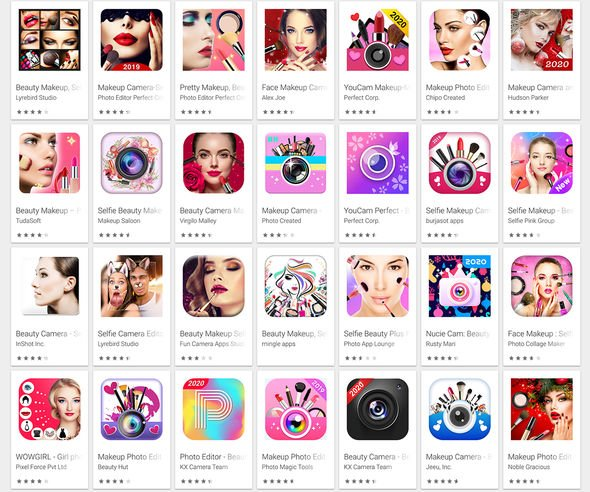
\includegraphics[trim=20 40 20 40,clip,width=0.9\textwidth]{chapter2/image/chplay.jpeg}
    \caption{Search results for "Beauty apps" on Google Play Store}
    \label{fig:android}
\end{figure}


\noindent Some features that make Android become much more popular than other smartphone operating system is:
\begin{itemize}
    \item 
	Android is highly customizable because it is an open-source operating system. It can be edited on its own without interference from Google. Can run on many devices with different processing architectures
\item	Java program language, which is chosen as main development, is easy to learn and write. Moreover, Java is a class-based and highly object-oriented program language so that it is able to accommodate big projects. Especially, Java has many powerful libraries; hence Android can take advantages from them.
\item	The developer community is large and supportive.
\end{itemize}

An Android app is shipped as an Android Package (APK) that contains different files. It contains the Android manifest specifying the app’s starting point, the executable code, the developer key, and the resources needed to run the app. If the app consists of any machine learning model, such models will be attached as a resource. After the app is packaged under the \emph{“.apk”} extension, an APK file can be public for users to download by using Google Play Store (has over 3 million apps are available there). \par

\subsection{AndroidX} \label{sec:androidx}

AndroidX is a major improvement to the original Android Support Library, which is no longer maintained. In other words, AndroidX provides new tools and libraries under the \verb|androix.*| namespace, while old packages taken from the Android Support Library are mapped to this new namespace. 
More supportive, all Jetpack components are packaged into AndroidX. Jetpack is a suite of libraries to help developers follow best practices, and make great Android apps that works consistently across Android versions and devices so that developers can focus on the code they care about. \par

\subsection{CameraX} \label{sec:camerax}

It is vital to handle cameras to get media data for the latter phases, capture the photos from the front or rear camera. Therefore, choosing an external library seems reasonable because it would be more reliable in case deploying in heterogeneous landscapes and device hardware. After investigating several camera libraries, such as camera2, PreviewCam, I choose CameraX as the app can make use of the Preview and Analysis user cases; thus, the app would reduce a substantial amount of code.\par

CameraX was first introduced in Google I/O 2019 as a Jetpack library, to meet the increased requirement of functionality for the camera. Meanwhile, the complexity and effort of the implementation would also be reduced considerably. CameraX inherits from Camera2 API, but with ease of use. It uses a simpler approach that is lifecycle-aware and is based on use cases. \par

CameraX's use cases allow you to focus on the task you need to accomplish instead of spending time covering device-specific settings. Three essential use cases of CameraX are: \par
\begin{itemize}
\item	Preview use case can be used to provide a preview of the current camera stream within a \emph{SurfaceTextureView}. This view is then connected to a corresponding \emph{TextureView} to display the camera content on screen. 
\item  Image analysis use case provides a CPU-accessible image to carry out image processing or machine learning inference. The image will be executed through the \emph{analyze()} method which runs on each frame.
\item	Image capture use case is used for low latency image captures. There are a number of options that we can set for the camera in this use case.
\end{itemize}


